\section{Definitions}
\label{sec:definitions}

One of the main reasons to introduce an ontology is to enable sharing of knowledge between researchers, developers, and users. 
Therefore, it is important that the terms we use are clearly defined. 
When presenting our ontology in \cref{sec:ontology}, we will formalize the terms such that they can be used by software agents.
In this section, we will define the terms linguistically, thereby providing insight into the terms used in the next section.
We will first define the concept of a scenario in \cref{sec:scenario}. 
Next, we will define two important attributes of a scenario: events and activities, in \cref{sec:event,sec:activity}, respectively. 
Lastly, we will present the definition of a scenario class in \cref{sec:scenario class}.

\cbstartc
In each of the \cref{sec:scenario,sec:event,sec:activity,sec:scenario class}, we start with some background information. Next, we draw few conclusions that lead to our proposed definition of the corresponding terms. After proposing a definition, we finish each section with some remarks and implications of our proposed definition.
\cbend



\subsection{Scenario}
\label{sec:scenario}

% Definition according to Go and Carroll
\textcite{go2004blind} describe a scenario within the field of system design. They define a scenario as ``a description that contains (1) actors, (2) background information on the actors and assumptions about their environment, (3) actors' goals or objectives, and (4) sequences of actions and events. Some applications may omit one of the elements or they may simply or implicitly express it. Although, in general, the elements of scenarios are the same in any field, the use of scenarios is quite different.'' 

% Definition according to Geyer et al.
\textcite{geyer2014} describe a scenario within the context of automated driving. They use the metaphor of a movie or a storybook for describing a scenario. \textcite{geyer2014} state that ``a scenario includes at least one situation within a scene including the scenery and dynamic elements. However, [a] scenario further includes the ongoing activity of one or both actors.'' For a further explanation of the terms situation, scene, and scenery, see \cite{geyer2014}. 
%It is mentioned that the action of the driver and/or automation might be predefined. 
In \cite{geyer2014}, the meaning of activity is not detailed.
%In an example of a so-called crossway scenario, they mention that the course of events might be different. For example, when a car keeps constant speed and then turns right, the scenario consists of one situation. The car might also first decelerate, accelerate and decelerate before turning right. In this case, the scenario consists of four situations.

% Definition according to Ulbrich et al.
\textcite{ulbrich2015} also define a scenario in the context of automated driving. They define a scenario as ``the temporal development between several scenes in a sequence of scenes. Every scenario starts with an initial scene. Actions \& events as well as goals \& values may be specified to characterize this temporal development in a scenario. Other than a scene, a scenario spans a certain amount of time.'' They state that actions and events link the different scenes. A further description of actions and events is not given in \cite{ulbrich2015}.

% Definition according to Elrofai et al.
Another definition of a scenario in the context of automated driving is given by \textcite{elrofai2016scenario}. They define a scenario as ``the combination of actions and maneuvers of the host vehicle in the passive [i.e., static] environment, and the ongoing activities and maneuvers of the immediate surrounding active [i.e., dynamic] environment for a certain period of time.'' They further mention that the duration of a scenario typically is in the order of seconds.

% What is missing in the definitions?
% 1. No difference between qualitative and quantitative. I.e., definitions are ambiguous.
% 2. There are undefined terms.
% 3. Definitions are not detailed enough to reflect into code.
\cbstart
Although the aforementioned definitions of scenario \cite{geyer2014, ulbrich2015, elrofai2016scenario} are in the context of automated driving, we require a more concrete definition. First, the aforementioned definitions do not specify the level of detail. 
%We experience much confusion where one group thinks a discussion is about a very specific scenario whereas another group thinks the same discussion is about a collection of scenarios that share some characteristics. 
Secondly, the aforementioned definitions use undefined terms, such as ``action'' and ``event''. Thirdly, because scenarios are used to specify test cases for the assessment of AVs, a clear and unambiguous specification of these scenarios is important and the aforementioned definitions are not concrete enough to be directly reflected into a coding language.
\cbend


% "Requirements"
Before providing the definition of the notion of scenario, characteristics of the notion of scenario are listed as follows:

% Order of seconds
\subsubsection{A scenario corresponds to a time interval}
The aforementioned definitions \cite{go2004blind, geyer2014, ulbrich2015, elrofai2016scenario} state that a scenario corresponds to a time interval. \textcite{vannotten2003updated} call such a scenario a chain scenario (``like movies''), as opposed to a snapshot scenario, i.e., a scenario that describes the state at a time instant (``like photos''). %The duration of a scenario is in the order of seconds, as explicitly mentioned by \textcite{elrofai2016scenario}. Though the duration is not mentioned by \textcite{ulbrich2015}, the presented example is in the order of seconds. Furthermore, other scenarios regarding (automated) driving are also in the order of seconds, e.g., see \cite{gietelink2006development, zofka2015datadrivetrafficscenarios, roesener2017comprehensive, karaduman2013interactivebehavior, hulshof2013autonomous, englund2016grand}.

% Scenarios consists of one or several events
\subsubsection{A scenario consists of one or several events \cite{vannotten2003updated, go2004blind, geyer2014, ulbrich2015, kahn1962, englund2016grand, schoemaker1993multiple, cuppens2002alert, bach2016modelbased}}
It can be helpful to develop scenarios using events \cite{bishop2007scentechniques}. Thus, a scenario could be defined as a particular sequence of events or, as \textcite[p.~143]{kahn1962} writes, ``a scenario results from an attempt to describe in more or less detail some hypothetical sequence of events''. Furthermore, \textcite{geyer2014} and \textcite{ulbrich2015} use the notion of event for describing a scenario, although they do not provide a definition of the term \emph{event}. In \cref{sec:event}, we will elaborate on the notion of \emph{event}.

% Semantically described
\subsubsection{Real-world traffic scenarios are quantitative scenarios}
Regarding the nature of the data, a scenario can be either qualitative or quantitative \cite{vannotten2003updated}. Real-world traffic scenarios are quantitative scenarios, such that they are, e.g., suitable for simulation purposes. A scenario, however, can also be described qualitatively, such that it is readable and understandable for human experts. Providing a qualitative description of a quantitative scenario has become known as a story-and-simulation approach \cite{alcamo2001scenarios}. Note that several quantitative scenarios might have the same qualitative description; thus, a qualitative description of a scenario does not uniquely define a quantitative scenario. A qualitative description can be regarded as an abstraction of the quantitative scenario.

% Some relevance between events
\subsubsection{The time interval of a scenario contains all relevant events}
According to \textcite{geyer2014}, ``the end of a scenario is defined by the first irrelevant situation with respect to the scenario''. In a similar manner, we require that the time interval of a scenario should contain all relevant events. Note that `relevant' is subjective and, therefore, an event is considered to be relevant, if it is relevant to the ego vehicle.
% Next to that, an event is regarded as irrelevant, if it is independent of the relevant events.

% Description of static environment
\subsubsection{A scenario includes the description of the environment}
A scenario should include the description of the static and dynamic environment.
Although the description of the static environment is not a general prerequisite of a scenario, this is often included when speaking about traffic scenarios \cite{geyer2014, ulbrich2015, elrofai2016scenario, ebner2011identifying, schuldt2013effiziente, althoff2017CommonRoad}.
%The static environment does not change during a scenario.
\cbstartc
The description of the dynamic environment includes a description of the type of actors and the goal and/or activities of the actors.
\cbend
%Everything that changes during the time interval of a scenario is considered to be part of the dynamic environment. 

% Goals (instead of activities)
\cbstartc
\subsubsection{A scenario describes the goal or activities of the ego vehicle}
For describing a scenario in real-world data, it is not necessary to describe the goals and therefore, \textcite{elrofai2016scenario} mention the activities of the ego vehicle rather than its goal. When describing a scenario that an AV has to cope with, however, its goals (i.e., its driving mission \cite{geyer2014}) could be specified rather than its activities \cite{ulbrich2015}. 
\cbend

% Definition
Hence, we define a scenario as follows:
\begin{definition}[Scenario]\label{def:scenario}
	A scenario is a quantitative description of the relevant characteristics of the ego vehicle, its activities and/or goals, its static environment, and its dynamic environment. From the perspective of the ego vehicle, a scenario contains all relevant events.
\end{definition}

% Describe difference from literature
% - quantitative --> to avoid ambiguous situation and to serve assessment
% - notion of scene not used. Scene follows from description, but is not explicitely used
\Cref{def:scenario} deviates from existing definitions \cite{geyer2014, ulbrich2015, elrofai2016scenario} in that it explicitly mentions that a scenario is quantitative. We use the term \emph{scenario class} to refer to the qualitative description, see \cref{sec:scenario class}.

\textcite{geyer2014} and \textcite{ulbrich2015} use the term \emph{scene} to define a scenario, while \cref{def:scenario} describes the scenes implicitly. Thus, the scenes do not have to be described explicitly.

\Cref{fig:scenario} shows a schematic overview of the various components of a scenario. As shown in the second row of \cref{fig:scenario}, a scenario contains an ego vehicle, a dynamic environment, and a static environment. As an example, possible activities of the vehicle in front, which is part of the dynamic environment, are detailed by considering the states `heading' and `speed'. Note that a definition of the term activity is given in \cref{sec:activity}. The two rows of the activities show more generic descriptions and more detailed descriptions, respectively, of some possible activities.

\begin{figure}
	\centering
	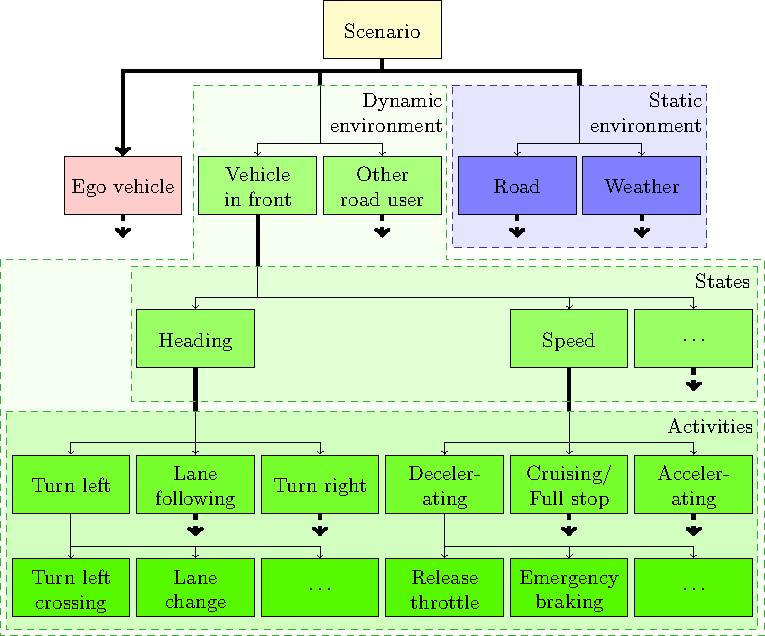
\includegraphics[width=\linewidth]{figures/scenario.pdf}%
	\caption{Schematic overview of a scenario. Note that the dynamic environment is not limited to the `vehicle in front', nor does it need to have the `vehicle in front'. Similarly, the static environment is not limited to `road', nor does it need to have `road'.}
	\label{fig:scenario}
\end{figure}

\cbstartb
According to \cref{def:scenario}, a scenario describes, among others, the static environment. When it comes to applying this definition in an ontology, it is possible that ``describing'' the static environment is done by simply providing a reference to a static environment. This also holds for the other parts of a scenario. \cbstartc The advantage of references is that these parts of the scenario can be exchanged between different scenarios, as these scenarios can use the same references. \cbend
As an example, an OpenSCENARIO file, which has as primary use case to describe the dynamic content of a scenario \cite{openscenario}, allows to provide a reference to an OpenDRIVE file which describes a road network \cite{dupuis2010opendrive}. As we will see in \cref{sec:ontology}, in our proposed ontology, a scenario contains references to a static environment, activities, actors, and events.
\cbend



\subsection{Event}
\label{sec:event}
% Introduction of this section
As mentioned in \cref{def:scenario}, a scenario consists of events. The notion of event is extensively used in literature \cite{breu1997towards, pfeiffer2013concepts, branicky1998hybridcontrol, deschutter2000optimal, heemels2012eventcontrol}. In this section, a selected number of descriptions is presented. Next, a definition of event is given that suits our context.

% Literature review
The term event is used in many different fields, e.g.:
\begin{itemize}
	\item In computing \cite{breu1997towards}, an event is an action or occurrence recognized by software. A common source of events are inputs by the software users. An event may trigger a state transition.
	%\item \textcite{kim1993supervenience}, a philosopher, writes: ``The term event ordinarily implies change''. \textcite{kim1993supervenience} states that an event is composed of three elements: objects, a property, and a time instant or a temporal interval. 
	\item In probability theory, an event is an outcome or a set of outcomes of an experiment \cite{pfeiffer2013concepts}. For example, a thrown coin landing on its tail is an event.
	%\item ``In relativity, an event is any occurrence with which a definite time and a definite location are associated; it is an idealization in the sense that any actual event is bound to have a finite extent both in time and in space'' \cite{sartori1996understanding}.
	\item In the field of hybrid theory, ``the continuous and discrete dynamics interact at `event' or `trigger' times when the continuous state hits certain prescribed sets in the continuous state space'' \cite{branicky1998hybridcontrol}. ``A hybrid system can be in one of several modes, [...], and the system switches from one mode to another due to the occurrence of events'' \cite{deschutter2000optimal}.
	\item In event-based control, a control action is computed when an event is triggered, as opposed to the more traditional approach where a control action is periodically computed \cite{heemels2012eventcontrol}. In event-based control, the event is triggered at the moment at which the system (is about to) reach a certain boundary.
\end{itemize}

Before providing the definition of an event, the following is concluded about an event:

% It is a time instant
\subsubsection{An event corresponds to a time instant}
Whether it is regarding computing, hybrid control, or event-based control, an event is happening at a time instant.

% Event should mark transition of a state from one set to another - mention relation with hybrid control
\subsubsection{An event marks a mode transition or the moment a system reaches a boundary}
A mode transition may be caused by either an abrupt change of an input signal, a change of a parameter, or a change in the model. For example, pushing the brake pedal may cause a mode transition and therefore, this may be regarded as an event. It is also possible that the event marks the moment that a system reaches a boundary. For example, a vehicle entering a tunnel, i.e., the distance between the vehicle and the tunnel reaches zero, can be an event.

%\subsubsection{An event marks (a cause of) a mode transition}
%Events mark the transition of mode, which is either a change of input, parameter or state. This is analogous to the way event is described in hybrid control \cite{boel1999hybridcontrol}.

% Give definition
Hence, we define an event as follows:
\begin{definition}[Event] \label{def:event}
	An event marks the time instant at which the system reaches a specified boundary or at which a mode transition occurs, such that before and after an event, the state of the system corresponds to two different modes.
\end{definition}

% Mention that there are basically two definitions. First definition more suitable for triggers for test cases. Second definition more suitable for observations and inputs. 
According to \cref{def:event}, an event occurs at either a moment at which the system reaches a boundary or a moment at which a mode transition occurs. 
\cbstart
Both these types of event are related to hybrid theory \cite{deschutter2003hybrid, heemels2012eventcontrol}.
The first type of event, i.e., at the moment at which the system reaches a boundary, is especially useful when describing test cases. For example, consider the ego vehicle approaching a pedestrian that is about to cross the road \cite{seiniger2015test}. Here, the event is at the moment that the distance between the vehicle and pedestrian is less than $\distancecondition$ meters. At this event, the pedestrian starts to cross the road such that the vehicle impacts the pedestrian if it does not change its speed or direction \cite{seiniger2015test}.
The second type of event, i.e., a mode transition, can be, for example, during an observed scenario at the moment at which a driver suddenly brakes. 

\cbstartb
For the practical implementation of events, a set of conditions may be specified. In that case, the event occurs at the moment that the conditions are met. A condition could be, for example, the distance between the vehicle and pedestrian. In \cite{openscenario}, an extensive list of possible conditions is given.
\cbend

%This first type of event, i.e., at the moment at which the system reaches a boundary, is related to events in event-based control \cite{heemels2012eventcontrol}, whereas the second type of event, i.e., at the moment at which a mode transition occurs, is related to events in hybrid theory \cite{deschutter2000optimal}. 
%Especially when designing scenarios for testing purposes, an event of the first type might trigger an event of the second type. For example, consider a vehicle approaching a zebra crossing with a pedestrian (dummy) that is about to cross the road at the zebra crossing. When the distance between the vehicle and the zebra crossing becomes less than 20 meters (event of the first type), the pedestrian (dummy) starts crossing the road at the zebra crossing (event of the second type).


%The inter-event time interval, i.e., the time in between two events, corresponds to a certain activity. For example, when the longitudinal acceleration is negative during an inter-event time interval, the activity can be described by the label `braking'.
%Another example of an event is the time instant at which the head lights are turned on. In that case, the activities before and after the event can be described as `lights off' and `lights on', respectively.



\subsection{Activity}
\label{sec:activity}

As mentioned in \cref{def:scenario}, a scenario \cbstartb includes \cbend a description of the dynamic environment of the ego vehicle. To describe the dynamic environment, activities are used. Furthermore, a scenario may describe the activities of the ego vehicle. Therefore, next to events, activities can be seen as the building blocks of a scenario.

\cbstart
Both the terms activity \cite{geyer2014, elrofai2018scenario, miller2015distraction, childress2015using, catapult2018musicc, sigsim2019glossary} and action \cite{geyer2014, ulbrich2015, bagschik2017ontology} are used in the context of automated driving. Although, strictly speaking, the terms action and activity have a slightly different meaning, it is often used for the same purpose:
\begin{itemize}
	\item According to \textcite{ulbrich2015}, actions may be specified for characterizing the temporal development in a scenario.
	\item \textcite{elrofai2018scenario} consider an activity as a building block of the dynamic part of the scenario: ``An activity is a time evolution of state variables such as speed and heading to describe for instance a lane change, or a braking-to-standstill.''
	\item In a glossary for a scenario catalog development \cite{catapult2018musicc}, an activity is defined as ``the state of an object over an interval of time. An activity starts with an event and ends with another event.''
%	\item According to the Cambridge Dictionary, an activity is defined as ``the doing of something, or something that you are doing, have done, or could do'' \cite{cambridge2019activity}.
%	\item \textcite{caspersen1985physical} define physical activity ``as any bodily movement produced by skeletal muscles that result in energy expenditure''.
%	\item \textcite{bobick1997movement} simply states that an activity is a ``sequence of movements''. 
\end{itemize}
\cbend

Before providing the definition of an activity, the following is concluded about an activity:

% Time interval
\subsubsection{An activity corresponds to an inter-event time interval}
As opposed to an event, an activity spans over a certain time interval. Furthermore, the start and the end of an activity is marked by an event.

% Describing the evolution of a state
\cbstart
\subsubsection{An activity quantitatively describes the time evolution of a state}
Because activities are building blocks of a scenario and a scenario corresponds to a quantitative description, the activities itself need to be quantitative as well. 
Therefore, an activity describes the time evolution of a state, i.e., the value(s) of a state over an inter-event time interval that corresponds to the activity, where the term state is defined in \cref{sec:state}.

% Performed by something (an actor?)
\subsubsection{An activity is performed by an actor}
An activity quantitatively describes the time evolution of a state and a state corresponds to an actor, e.g., the acceleration of a vehicle, and, therefore, an activity is performed by an actor. Note that the actor might be the ego vehicle. 
%However, it might also be the case that a state does not correspond to an actor. For example, a state describing the weather conditions does not correspond to an actor, so if an activity describes changing weather conditions, the activity is not performed by an actor.

Hence, we define an activity as follows:
\begin{definition}[Activity]
	\label{def:activity}
	An activity quantitatively describes the time evolution of a state of an actor between two events.
\end{definition}
\cbend

% Remarks
% 1. Activity is very similar to mode, i.e., a model that describes the evolution of a state over time with parameters theta
% Skipped...

% 2. Activity vs. action
Note that \textcite{geyer2014, ulbrich2015} use the term \emph{action} and although they do not define this term, it seems to be related to our use of the term activity. Similarly, other authors \cite{sigsim2019glossary, catapult2018musicc, elrofai2018scenario} use the term activity. Although the terms \emph{activity} and \emph{action} may seem very similar, there is a difference. As \textcite{bobick1997movement} points out, actions require an interpretive context --- ``a set of constraints on possible explanations for the observed motions.'' In our case, we do not want to bother ourselves with detailing on the purpose of each of the activities. Hence, we refrain from using the term \emph{action}.

% 3. Examples of activities
Examples of activities are accelerating, cruising, and decelerating. Here, the activities describe the longitudinal acceleration (or, e.g., speed). Activities describing the lateral position of a vehicle with respect to the center of the \cbstartb corresponding lane \cbend might, for example, be labeled with ``driving straight'' or ``lane change''.



\subsection{Scenario class}
\label{sec:scenario class}

% Introduce term scenario class (i.e. qualitative description of scenario)
\cbstart
As proposed in \cref{def:scenario}, a scenario in the context of the performance assessment of an AV needs to be quantitative. 
However, in literature, the term scenario is also used to refer to a collection of scenarios, where this collection of scenarios is semantically described. For example, in \cite{USDoT2007precrashscenarios}, a typology of pre-crash scenarios is proposed. Here, each of the pre-crash scenarios is an abstraction of many quantitative scenarios. Similar studies are performed to describe scenarios that lead to highway accidents \cite{adaptive2017d73}, car-cyclist accidents \cite{opdencamp2014cats}, and car-pedestrian accidents \cite{lenard2011typical}. In \cite{catapult2017taxonomy}, a taxonomy of scenarios is proposed to qualitatively describe challenging scenarios for automated driving.

The aforementioned references \cite{USDoT2007precrashscenarios, adaptive2017d73, opdencamp2014cats, lenard2011typical, catapult2017taxonomy} show that the term \emph{scenario} is also used to address qualitative descriptions. Since we defined a scenario as a quantitative description, we need to introduce a different term to address the qualitative description. We propose to use the term \emph{scenario class} to refer to the qualitative description of a scenario. A qualitative description can be regarded as an abstraction of a quantitative scenario, \cbstartb whereas a quantitative description can be regarded as a concretization of a qualitative description.
\cbend
%However, each scenario can be abstractly described in words; i.e., a qualitative description of each scenario exists. 
%Therefore, a scenario class refers to multiple scenarios with a common characteristic \cite{elrofai2018scenario}.

We define a scenario class as follows:
\begin{definition}[Scenario class] \label{def:scenario class}
	A scenario class is a qualitative description of the ego vehicle, its activities and/or goals, its static environment, and its dynamic environment.
\end{definition}

% What is the purpose of this?
% - Human interpretable
% - Group scenarios that are very similar --> Analysis is easier
% - Completeness
Introducing the concept of scenario classes brings the following benefits:
\begin{itemize}
	\item For a human, it is easier to interpret a qualitative description rather than a quantitative description.
	\item It enables to refer to a group of scenarios that have something in common. Therefore, it enables characterization of the type of scenarios, thus making discussing scenarios much easier.
	\item It enables easier comparison of scenarios. This can be used to quantify the completeness of a set of scenarios; see \cite{degelder2019completeness} for more details on this.
\end{itemize}

% Explain scenarios fall into scenario class
We describe the formal relation between a scenario and a scenario class with the verb ``to fall into'', denoted by $\scenariofallsinto$. If a specific scenario class $\scenarioclass$ is an abstraction of a specific scenario $\scenario$, then we say that the specific scenario $\scenario$ falls into that specific scenario class $\scenarioclass$, or simply $\scenario \scenariofallsinto \scenarioclass$. \cbstartc This is illustrated in \cref{fig:venn diagram scenario class}, where $\scenarioa$, $\scenariob$, and $\scenarioc$ represent scenarios and $\scenarioclassa$, $\scenarioclassb$, and $\scenarioclassc$ represent scenario classes. Multiple scenarios can fall into a given scenario class. For example, we have $\scenarioa \scenariofallsinto \scenarioclassb$ and $\scenariob \scenariofallsinto \scenarioclassb$ in \cref{fig:venn diagram scenario class}. 
% Explain scenario can fall into multiple scenario classes
Furthermore, a scenario can fall into multiple scenario classes. For example, in \cref{fig:venn diagram scenario class}, we have $\scenariob \scenariofallsinto \scenarioclassa$, $\scenariob \scenariofallsinto \scenarioclassb$, and $\scenariob \scenariofallsinto \scenarioclassc$.
\cbend
%Whereas multiple scenarios can fall into one scenario class, it is also possible for one scenario to fall into multiple scenario classes. Continuing the example of \cref{fig:venn diagram scenario class}, a scenario with rain during daytime falls into both the scenario classes ``Daytime'' and ``Rain''.

\setlength{\venncircle}{7em}
\begin{figure}
	\centering
	\begin{tikzpicture}
	% Circles
	\fill[red, fill opacity=0.5] (-\venncircle/2, 0) circle (\venncircle);
	\fill[green, fill opacity=0.5] (\venncircle/2, 0) circle (\venncircle);
	\draw (-\venncircle/2, 0) circle (\venncircle);
	\draw (\venncircle/2, 0) circle (\venncircle);
	
	% Names of scenario classes
	\node[anchor=east](daylight) at (-5/4*\venncircle, \venncircle) {$\scenarioclassb$};
	\draw (daylight) -- ({(-sqrt(2)/2-1/2)*\venncircle}, {sqrt(2)/2*\venncircle});
	\node[anchor=west](rain) at (5/4*\venncircle, \venncircle) {$\scenarioclassc$};
	\draw (rain) -- ({(sqrt(2)/2+1/2)*\venncircle}, {sqrt(2)/2*\venncircle});
	\node[anchor=south](day and rain) at (-1/4*\venncircle, 8/7*\venncircle) {$\scenarioclassa$};
	\draw (day and rain) -- ({(1/2-sqrt(2)/2)*\venncircle}, {(sqrt(2)/2)*\venncircle});
	
	% Scenarios
	\node at (-0.1*\venncircle, -0.1*\venncircle) (scenariob){\textbullet};
	\node at (-\venncircle, 0.3*\venncircle) (scenarioa){\textbullet};
	\node at (\venncircle, 0.2*\venncircle) (scenarioc){\textbullet};
	\node[right of=scenarioa, node distance=1em]{$\scenarioa$};
	\node[right of=scenariob, node distance=1em]{$\scenariob$};
	\node[right of=scenarioc, node distance=1em]{$\scenarioc$};
	%\node[text width=\venncircle, align=center] at (-\venncircle, 0) {Scenarios without rain during daytime};
	%\node[text width=\venncircle, align=center] at (0, 0) {Scenarios with rain during daytime};
	%\node[text width=.9\venncircle, align=center] at (\venncircle, 0) {Scenarios with rain during nighttime};
\end{tikzpicture}

	\caption{\cbstartc The red and green circles correspond to the scenario classes $\scenarioclassb$ and $\scenarioclassc$, respectively. The overlap between the two circles corresponds to scenario class $\scenarioclassa$. The dots represent scenarios $\scenarioa$, $\scenariob$, and $\scenarioc$. Scenarios $\scenarioa$ and $\scenariob$ fall into scenario class $\scenarioclassb$. Scenario class $\scenarioclassa$ falls into scenario classes $\scenarioclassb$ and $\scenarioclassc$.\cbend}
	\label{fig:venn diagram scenario class}
\end{figure}

% Explain scenario class can fall into scenario classes
The verb ``to fall into'' is also used to describe the relation between two scenario classes. A scenario class $\scenarioclassa$ is said to fall into a scenario class $\scenarioclassb$ if all scenarios that fall into scenario class $\scenarioclassa$ also fall into scenario class $\scenarioclassb$. In that case, we can write $\scenarioclassa \scenarioclassfallsinto \scenarioclassb$. Thus we have
\begin{equation} \label{eq:fall into scenario class}
	\scenarioclassa \scenarioclassfallsinto \scenarioclassb \text{ if } \scenario \scenariofallsinto \scenarioclassb \,\,\forall\,\, \scenario \scenariofallsinto \scenarioclassa.
\end{equation}
\cbstartc
In \cref{fig:venn diagram scenario class}, scenario class $\scenarioclassa$ falls into scenario classes $\scenarioclassb$ and $\scenarioclassc$, thus $\scenarioclassa \scenarioclassfallsinto \scenarioclassb$ and $\scenarioclassa \scenarioclassfallsinto \scenarioclassc$.
\cbend
%In \cref{fig:venn diagram scenario class}, an example is shown with the scenario class ``Rain during daytime'', which falls into the scenario classes ``Daytime'' and ``Rain''.
%For example, consider the scenario class ``Rain during day'', which is represented by the intersection of the red and green circles in \cref{fig:venn diagram scenario class}. All scenarios with rain that occur during the day fall into this scenario class. Obviously, these scenarios also fall into the scenario classes ``Day'' and ``Rain''. Hence, the scenario class ``Rain during day'' falls into the scenario classes ``Day'' and ``Rain''.

When providing extra information on a piece of data, often tags are used \cite{smith2007tagging}. A tag is a keyword or a term that helps describing an item. For example, items in a database can contain some tags that enable users to quickly obtain several items that share a certain characteristic described by a tag \cite{craft2004tagging, vasquez2019controlling}. Applications are very broad, e.g., from classification of audio data \cite{kong2017joint} and capturing musical characteristics from songs \cite{ellis2011semantic} to tagging of Wikipedia pages \cite{voss2006collaborative}.

% Figure is explained in last few paragraphs, but placed earlier as to appear at the right page of the paper.
\begin{figure*}
	\centering
	\begin{subfigure}{\linewidth}
		\centering
		\tree{Vehicle lateral activity}{Going straight; Changing lane, Left, Right; Turning, Left, Right; Swerving, Left, Right}
		\caption{Lateral activities of a vehicle.}
		\label{fig:tree vehicle lat act}
	\end{subfigure}
	\begin{subfigure}{\linewidth}
		\centering
		\tree{Vehicle longitudinal activity}{Reversing; Standing still; Driving forward, Braking, Cruising, Accelerating}
		\caption{Longitudinal activities of a vehicle.}
		\label{fig:tree vehicle long act}
	\end{subfigure}
	\caption{Tags for lateral and longitudinal activities of a vehicle. The lateral activity is relative to the lane in which the corresponding vehicle is driving.}
	\label{fig:tree vehicle activities}
\end{figure*}

\cbstartc We propose to provide scenarios and scenario classes with additional information in the form of tags that describe the scenario in a qualitative manner.
The tags of a scenario can be used to determine which scenario classes the scenario falls into.
%For example, if a scenario contains the tag ``Daytime'', it is automatically recognized as a scenario that falls into the scenario class ``Daytime'' which is characterized by the single tag ``Daytime''. 
\cbend
The use of these tags brings some benefits:
\begin{itemize}
	\item The scenarios do not need to be explicitly classified. Classifying scenarios can be a time-consuming effort if the number of scenario classes is high.
	\item If a scenario class that only contains known tags is added to the database of scenario classes, it can easily be seen which scenarios fall into this scenario class by only inspecting the tags of the scenarios. Therefore, there is no need to define scenario classes a priori.
	\item It is easy to select scenarios from a scenario database or a scenario library by using tags or a combination of tags.
	\item As opposed to the proposed categorization of scenarios in \cite{opdencamp2014cats, USDoT2007precrashscenarios, lenard2011typical, lara2019harmonized}, scenario classes do not need to be mutually exclusive.
\end{itemize}

There is a balance between having generic scenario classes - and thus a wide variety among the scenarios belonging to the scenario class - and having specific scenario classes without much variety among the scenarios in the scenario class. For some systems, one may be interested in very specific set of scenarios, while for another system one might be interested in a set of scenarios with a high variety. To accommodate this, tags are structured in hierarchical trees \cite{molloy2017dynamic, badger2012dynamic}. The different layers of the trees can be regarded as different abstraction levels \cite{Bonnin2014}. 

In \cite{degelder2019scenarioclasses}, several trees of tags are defined and \cref{fig:tree vehicle activities} shows two examples of trees of tags taken from \cite{degelder2019scenarioclasses}. These tags describe possible activities of a vehicle, i.e., the lateral motion control (via steering) and longitudinal motion control (via acceleration and deceleration) are reflected into tags. The tags may refer to the objective of an actor in case no activities are defined. For example, a test case in which the ego vehicle's objective is to make a left turn, the tags ``Turning'' and ``Left'' are applicable. 

Four different types of activities are identified regarding the lateral movement, see \cref{fig:tree vehicle lat act}. Here, it is assumed that ``Lateral'' refers to the direction perpendicular to the lane the vehicle is driving in (e.g., according to the Road Coordinate System in \cite{zofka2015datadrivetrafficscenarios}). Therefore, if the vehicle is driving on a curved road while staying more or less in its lane (lane-following), the tag ``Going straight'' is applicable. Apart from going straight, the vehicle might change lane, turn, or swerve to either the left or the right.

